\documentclass[aspectratio=169]{beamer}

\usetheme{default}
\usecolortheme{dove}

\setbeamertemplate{navigation symbols}{}
\setbeamertemplate{footline}{%
  \hfill{\large\insertframenumber\,/\,\inserttotalframenumber}\hspace{0.8em}\vspace{0.5em}%
}

\definecolor{popblue}{RGB}{52, 101, 164}
\definecolor{sampred}{RGB}{204, 0, 0}
\definecolor{paramgreen}{RGB}{0, 140, 70}
\definecolor{warnred}{RGB}{180, 40, 40}
\definecolor{orange1}{RGB}{220, 120, 0}
\definecolor{violet1}{RGB}{120, 50, 160}
\definecolor{lightbg}{RGB}{245, 245, 250}

\setbeamercolor{frametitle}{fg=popblue}
\setbeamercolor{title}{fg=popblue}

\usepackage{pgfplots}
\usepackage{tikz}
\usetikzlibrary{shapes, arrows.meta, positioning, calc, decorations.pathreplacing, patterns}
\pgfplotsset{compat=1.18}
\usepackage{amsmath, amssymb}
\usepackage{fontenc}

\title{Lecture 5: Point Estimation}
\subtitle{Method of Moments $\cdot$ Maximum Likelihood $\cdot$ Why MLE Works}
\date{}

\begin{document}

% ============================================================
\begin{frame}
\titlepage
\end{frame}

% ============================================================
\begin{frame}
\frametitle{Previously, on Lecture 4\ldots}

\begin{center}
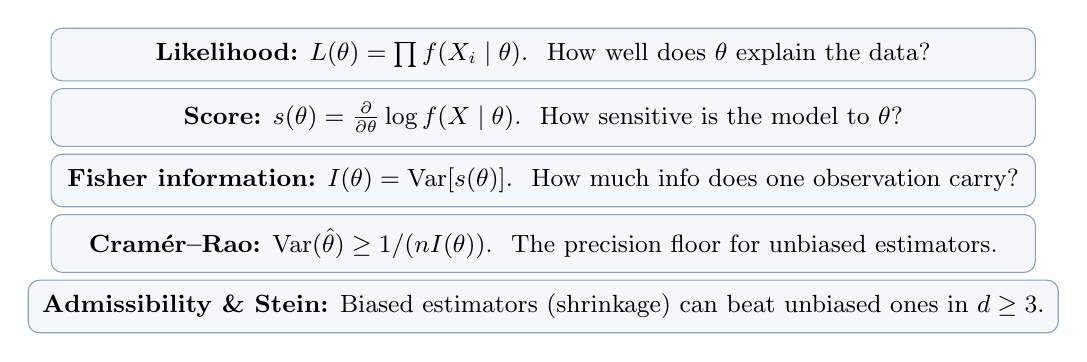
\begin{tikzpicture}[
  sbox/.style={draw=popblue!60, fill=popblue!5, rounded corners=4pt, minimum width=12.5cm, minimum height=0.5cm, align=left, inner sep=5pt, font=\small}
]
  \node[sbox] at (0, 2.0) {\textbf{Likelihood:} $L(\theta) = \prod f(X_i \mid \theta)$. \;How well does $\theta$ explain the data?};
  \node[sbox] at (0, 1.2) {\textbf{Score:} $s(\theta) = \frac{\partial}{\partial\theta}\log f(X \mid \theta)$. \;How sensitive is the model to $\theta$?};
  \node[sbox] at (0, 0.4) {\textbf{Fisher information:} $I(\theta) = \text{Var}[s(\theta)]$. \;How much info does one observation carry?};
  \node[sbox] at (0, -0.4) {\textbf{Cram\'er--Rao:} $\text{Var}(\hat\theta) \geq 1/(nI(\theta))$. \;The precision floor for unbiased estimators.};
  \node[sbox] at (0, -1.2) {\textbf{Admissibility \& Stein:} Biased estimators (shrinkage) can beat unbiased ones in $d \geq 3$.};
\end{tikzpicture}
\end{center}

\vspace{0.3cm}
\begin{center}
{\large\textbf{Today:}} We know how to \textbf{judge} estimators. Now: how to \textbf{construct} them.\\[4pt]
Two systematic recipes: \textbf{Method of Moments} and \textbf{Maximum Likelihood}.
\end{center}
\end{frame}

% ============================================================
\begin{frame}
\frametitle{The Estimation Problem}
\begin{center}
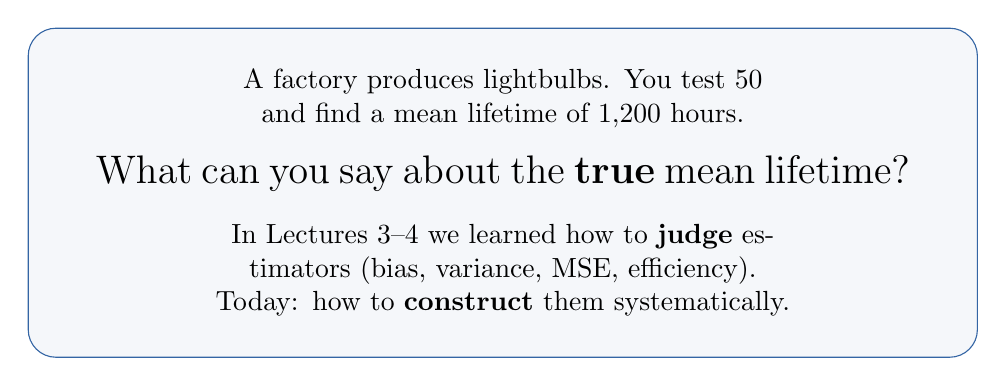
\begin{tikzpicture}
  \node[draw=popblue, fill=popblue!5, rounded corners=10pt, text width=11cm, align=center, inner sep=15pt] {
    A factory produces lightbulbs. You test 50 and find a mean lifetime of 1{,}200 hours.\\[10pt]
    {\Large What can you say about the \textbf{true} mean lifetime?}\\[10pt]
    In Lectures~3--4 we learned how to \textbf{judge} estimators (bias, variance, MSE, efficiency).\\
    Today: how to \textbf{construct} them systematically.
  };
\end{tikzpicture}
\end{center}
\end{frame}

\begin{frame}
\frametitle{From Data to Parameters}
\begin{center}
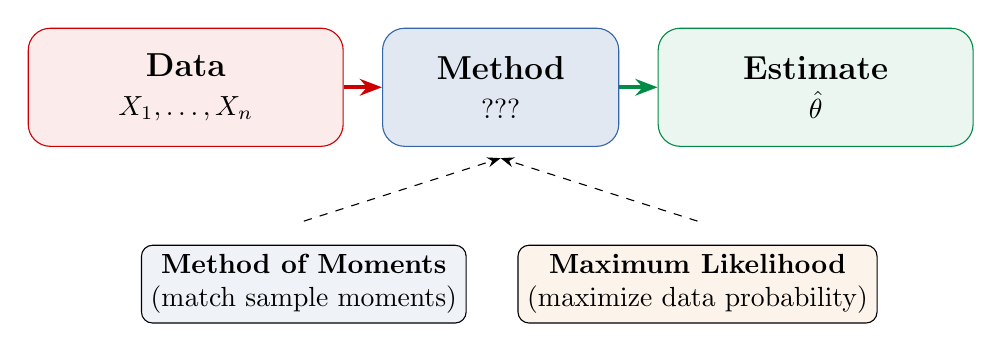
\begin{tikzpicture}[
  arrow/.style={-{Stealth[length=8pt]}, line width=1.5pt}
]
  % Data
  \node[draw=sampred, fill=sampred!8, rounded corners=8pt, minimum width=4cm, minimum height=1.5cm, font=\large\bfseries, align=center] (data) at (-4, 0) {Data\\{\normalsize\normalfont $X_1, \ldots, X_n$}};

  % Black box
  \node[draw=popblue, fill=popblue!15, rounded corners=8pt, minimum width=3cm, minimum height=1.5cm, font=\large\bfseries, align=center] (method) at (0, 0) {Method\\{\normalsize\normalfont ???}};

  % Estimate
  \node[draw=paramgreen, fill=paramgreen!8, rounded corners=8pt, minimum width=4cm, minimum height=1.5cm, font=\large\bfseries, align=center] (est) at (4, 0) {Estimate\\{\normalsize\normalfont $\hat{\theta}$}};

  \draw[arrow, sampred] (data) -- (method);
  \draw[arrow, paramgreen] (method) -- (est);

  % Two methods below
  \node[draw, rounded corners=4pt, fill=popblue!8, minimum width=4cm, font=\normalsize, align=center] at (-2.5, -2.5) {\textbf{Method of Moments}\\(match sample moments)};
  \node[draw, rounded corners=4pt, fill=orange1!8, minimum width=4cm, font=\normalsize, align=center] at (2.5, -2.5) {\textbf{Maximum Likelihood}\\(maximize data probability)};

  \draw[-{Stealth}, dashed] (-2.5, -1.7) -- (0, -0.9);
  \draw[-{Stealth}, dashed] (2.5, -1.7) -- (0, -0.9);
\end{tikzpicture}
\end{center}
\end{frame}

% ============================================================
\section{Method of Moments}

\begin{frame}
\frametitle{Method of Moments (MoM)}

\textbf{Idea:} Set population moments equal to sample moments, then solve for the parameters.

\vspace{0.4cm}
\begin{center}
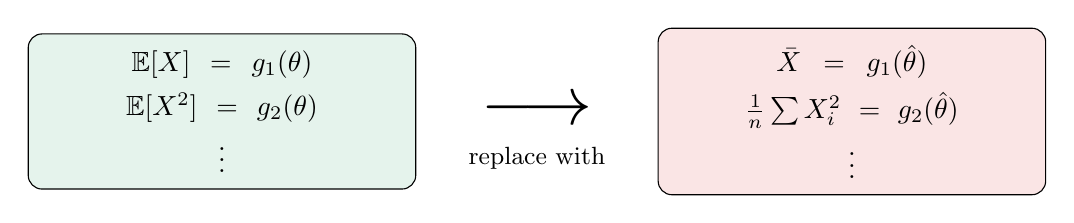
\begin{tikzpicture}[
  mombox/.style={draw, rounded corners=5pt, minimum height=1cm, text width=4.5cm, align=center, font=\normalsize, inner sep=6pt}
]
  \node[mombox, fill=paramgreen!10] at (-4, 0) {
    $\mathbb{E}[X] = g_1(\theta)$\\[4pt]
    $\mathbb{E}[X^2] = g_2(\theta)$\\[2pt]
    $\vdots$
  };

  \node[font=\Huge] at (0, 0) {$\longrightarrow$};
  \node[font=\small] at (0, -0.6) {replace with};

  \node[mombox, fill=sampred!10] at (4, 0) {
    $\bar{X} = g_1(\hat{\theta})$\\[4pt]
    $\frac{1}{n}\sum X_i^2 = g_2(\hat{\theta})$\\[2pt]
    $\vdots$
  };
\end{tikzpicture}
\end{center}

\vspace{0.3cm}
\pause
\begin{columns}
\begin{column}{0.48\textwidth}
  \textcolor{paramgreen}{\textbf{Pros:}}
  \begin{itemize}\small
    \item Simple, quick to compute
    \item No distributional assumption needed for computation
  \end{itemize}
\end{column}
\begin{column}{0.48\textwidth}
  \textcolor{warnred}{\textbf{Cons:}}
  \begin{itemize}\small
    \item Can give impossible values (e.g., $\hat{\sigma}^2 < 0$)
    \item Generally less efficient than MLE
    \item Awkward with many parameters
  \end{itemize}
\end{column}
\end{columns}
\end{frame}

\begin{frame}
\frametitle{MoM Example: Normal Distribution}
\begin{center}
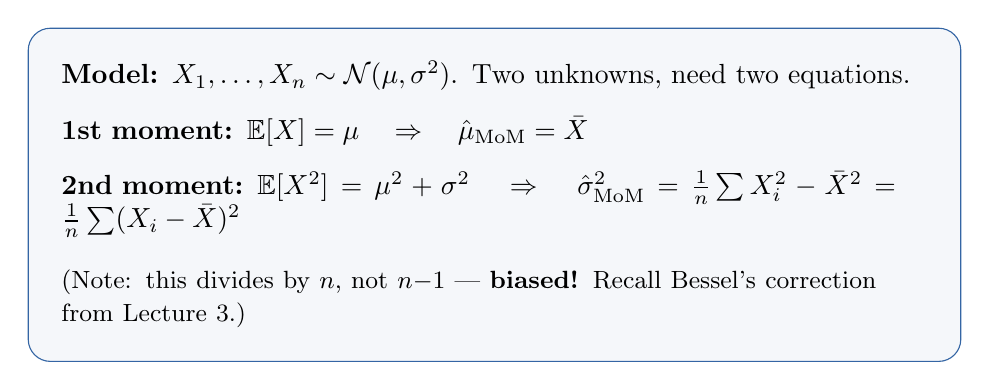
\begin{tikzpicture}
  \node[draw=popblue, fill=popblue!5, rounded corners=8pt, text width=11cm, align=left, inner sep=12pt] {
    \textbf{Model:} $X_1, \ldots, X_n \sim \mathcal{N}(\mu, \sigma^2)$. Two unknowns, need two equations.\\[8pt]
    \textbf{1st moment:} $\mathbb{E}[X] = \mu \quad\Rightarrow\quad \hat{\mu}_{\text{MoM}} = \bar{X}$\\[8pt]
    \textbf{2nd moment:} $\mathbb{E}[X^2] = \mu^2 + \sigma^2 \quad\Rightarrow\quad \hat{\sigma}^2_{\text{MoM}} = \frac{1}{n}\sum X_i^2 - \bar{X}^2 = \frac{1}{n}\sum(X_i - \bar{X})^2$\\[10pt]
    \small (Note: this divides by $n$, not $n{-}1$ --- \textbf{biased!} Recall Bessel's correction from Lecture~3.)
  };
\end{tikzpicture}
\end{center}
\end{frame}

\begin{frame}
\frametitle{When MoM Goes Wrong}

\small
MoM can give \textbf{impossible} parameter values because it doesn't ``know'' the constraints.

\vspace{0.2cm}
\textbf{Example:} Fit a $\text{Uniform}(0, \theta)$ distribution using MoM.

\vspace{0.1cm}
\quad Population mean: $\mathbb{E}[X] = \theta/2$ \quad$\Rightarrow$\quad $\hat\theta_{\text{MoM}} = 2\bar{X}$

\pause
\vspace{0.15cm}
\textbf{Problem:} We need $\hat\theta \geq \max(X_i)$, but MoM doesn't enforce this!

\vspace{0.1cm}
\begin{center}
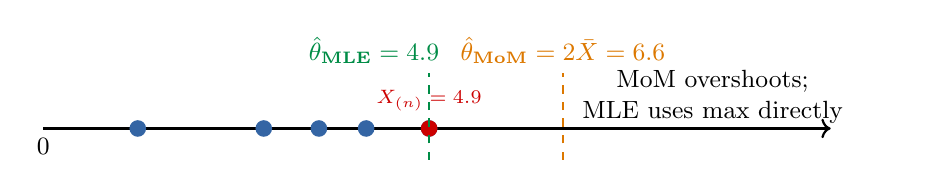
\begin{tikzpicture}
  \draw[thick, ->] (0, 0) -- (10, 0) node[right, font=\small] {};
  \node[below, font=\small] at (0, 0) {$0$};

  % Data points
  \foreach \x in {1.2, 2.8, 3.5, 4.1, 4.9} {
    \fill[popblue] (\x, 0) circle (3pt);
  }
  \fill[sampred] (4.9, 0) circle (3pt);
  \node[above, font=\scriptsize, sampred] at (4.9, 0.1) {$X_{(n)} = 4.9$};

  % MoM estimate
  \draw[thick, dashed, orange1] (6.6, -0.4) -- (6.6, 0.7);
  \node[above, font=\small\bfseries, orange1] at (6.6, 0.7) {$\hat\theta_{\text{MoM}} = 2\bar{X} = 6.6$};

  % MLE estimate
  \draw[thick, dashed, paramgreen] (4.9, -0.4) -- (4.9, 0.7);
  \node[above, font=\small\bfseries, paramgreen] at (4.2, 0.7) {$\hat\theta_{\text{MLE}} = 4.9$};

  \node[font=\small, text width=5cm, align=center] at (8.5, 0.4) {MoM overshoots;\\MLE uses max directly};
\end{tikzpicture}
\end{center}

\vspace{0.1cm}
\centering\small MoM doesn't use the data efficiently here --- it ignores the maximum, which is the sufficient statistic.
\end{frame}

% ============================================================
\section{Likelihood}

\begin{frame}
\frametitle{The Likelihood Function (Recap from Lecture 4)}

\small
\begin{center}
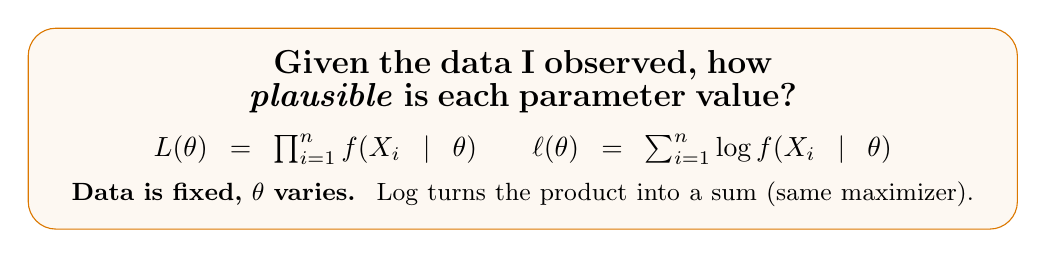
\begin{tikzpicture}
  \node[draw=orange1, fill=orange1!5, rounded corners=10pt, text width=12cm, align=center, inner sep=8pt] {
    {\large\bfseries Given the data I observed, how \textit{plausible} is each parameter value?}\\[6pt]
    $L(\theta) = \prod_{i=1}^n f(X_i \mid \theta) \qquad \ell(\theta) = \sum_{i=1}^n \log f(X_i \mid \theta)$\\[4pt]
    \small \textbf{Data is fixed, $\theta$ varies.} \;Log turns the product into a sum (same maximizer).
  };
\end{tikzpicture}
\end{center}

\vspace{0.1cm}
\pause
From Lecture~4, we already know:
\begin{itemize}\setlength{\itemsep}{1pt}
  \item The \textbf{score} $s(\theta) = \ell'(\theta)$ measures sensitivity to $\theta$; \;$\mathbb{E}[s] = 0$
  \item \textbf{Fisher information} $I(\theta) = \text{Var}[s] = -\mathbb{E}[\ell'']$ measures the curvature
  \item \textbf{Cram\'er--Rao:} no unbiased estimator can have $\text{Var} < 1/(nI(\theta))$
\end{itemize}

\vspace{0.05cm}
\centering Now: how to \textbf{use} the likelihood to actually \textbf{construct} estimators.
\end{frame}

\begin{frame}
\frametitle{Likelihood: Coin Flip Example}
\begin{center}
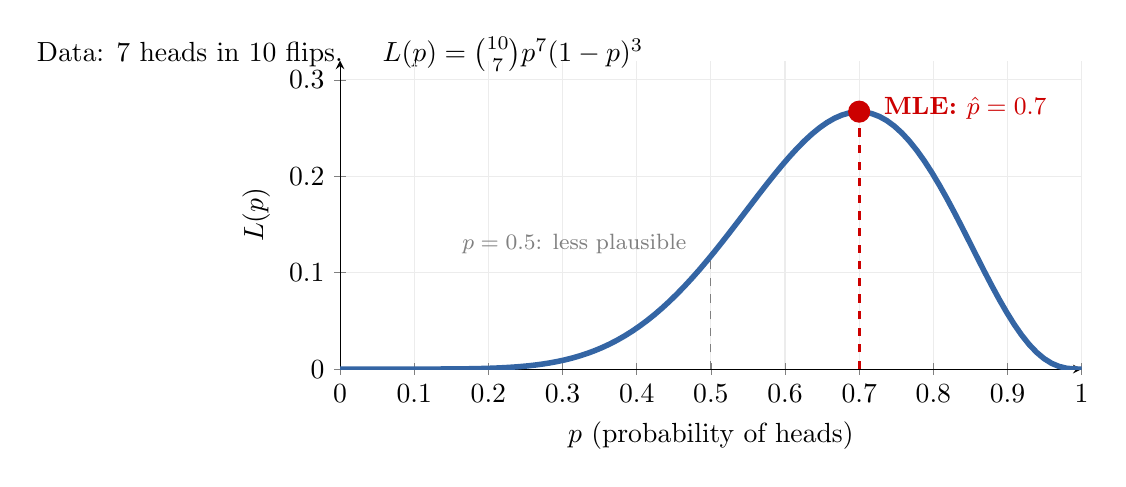
\begin{tikzpicture}
  \node[font=\normalsize] at (0, 4) {Data: 7 heads in 10 flips. \quad $L(p) = \binom{10}{7} p^7 (1-p)^3$};

  \begin{axis}[
    width=11cm, height=5.5cm,
    xlabel={$p$ (probability of heads)},
    ylabel={$L(p)$},
    xmin=0, xmax=1,
    ymin=0, ymax=0.32,
    axis lines=left,
    grid=major, grid style={gray!15},
    every axis plot/.append style={line width=2pt, samples=100}
  ]
    \addplot[popblue, domain=0:1] {120 * x^7 * (1-x)^3};

    % MLE marker
    \draw[very thick, sampred, dashed] (axis cs:0.7, 0) -- (axis cs:0.7, 0.267);
    \fill[sampred] (axis cs:0.7, 0.267) circle (4pt);
    \node[font=\small\bfseries, sampred, right] at (axis cs:0.72, 0.27) {MLE: $\hat{p} = 0.7$};

    % Other values
    \draw[thin, dashed, gray] (axis cs:0.5, 0) -- (axis cs:0.5, 0.117);
    \node[font=\footnotesize, gray, left] at (axis cs:0.48, 0.13) {$p=0.5$: less plausible};
  \end{axis}
\end{tikzpicture}
\end{center}
\end{frame}

\begin{frame}
\frametitle{The MLE Idea: What Would the Data Choose?}

\small
Imagine you could ask the data: ``Which parameter value explains you best?''

\vspace{0.2cm}
\begin{center}
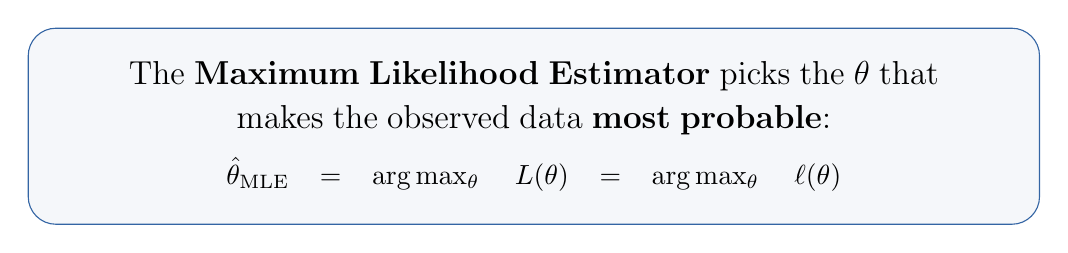
\begin{tikzpicture}
  \node[draw=popblue, fill=popblue!5, rounded corners=10pt, text width=12cm, align=center, inner sep=12pt] {
    {\large The \textbf{Maximum Likelihood Estimator} picks the $\theta$ that\\[4pt]
    makes the observed data \textbf{most probable}:}\\[8pt]
    $\hat{\theta}_{\text{MLE}} = \arg\max_\theta \; L(\theta) = \arg\max_\theta \; \ell(\theta)$
  };
\end{tikzpicture}
\end{center}

\vspace{0.2cm}
\pause
\textbf{Intuition:} If you flip a coin 10 times and get 7 heads\ldots
\begin{itemize}\setlength{\itemsep}{2pt}
  \item Is $p = 0.5$ plausible? Somewhat.
  \item Is $p = 0.7$ plausible? Very --- it predicts exactly what you saw.
  \item Is $p = 0.99$ plausible? Not really --- you'd expect more heads.
\end{itemize}

\vspace{0.1cm}
MLE picks $\hat{p} = 0.7$ because it maximizes the likelihood $L(p) = \binom{10}{7}p^7(1-p)^3$.

\vspace{0.1cm}
\centering\small At the MLE: $s(\hat\theta) = 0$ (score equals zero --- first-order condition from Lecture~4).
\end{frame}

% ============================================================
\section{Maximum Likelihood Estimation}

\begin{frame}
\frametitle{MLE Recipe: Step by Step}

\small
In practice, finding the MLE is a calculus exercise:

\vspace{0.2cm}
\begin{center}
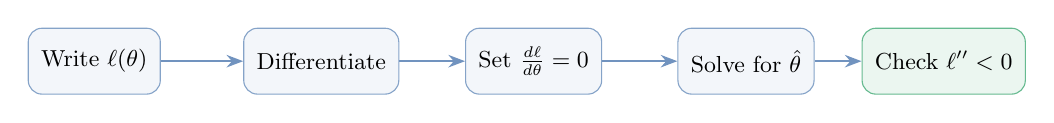
\begin{tikzpicture}[scale=0.93, every node/.style={transform shape},
  stp/.style={draw=popblue!60, fill=popblue!6, rounded corners=5pt, minimum height=0.9cm, align=center, inner sep=5pt, font=\small},
  arr/.style={-{Stealth[length=6pt]}, thick, popblue!70}
]
  \node[stp] (s1) at (0, 0) {Write $\ell(\theta)$};
  \node[stp] (s2) at (3.1, 0) {Differentiate};
  \node[stp] (s3) at (6.0, 0) {Set $\frac{d\ell}{d\theta} = 0$};
  \node[stp] (s4) at (8.9, 0) {Solve for $\hat\theta$};
  \node[stp, fill=paramgreen!8, draw=paramgreen!60] (s5) at (11.6, 0) {Check $\ell'' < 0$};
  \draw[arr] (s1) -- (s2);
  \draw[arr] (s2) -- (s3);
  \draw[arr] (s3) -- (s4);
  \draw[arr] (s4) -- (s5);
\end{tikzpicture}
\end{center}

\pause
\vspace{0.3cm}
\begin{columns}[T]
\begin{column}{0.48\textwidth}
\textbf{When it's easy} (closed form):
\begin{itemize}\setlength{\itemsep}{2pt}
  \item Exponential families
  \item Normal, Bernoulli, Poisson, Exp
  \item Solve $s(\hat\theta) = 0$ by hand
\end{itemize}
\end{column}
\begin{column}{0.48\textwidth}
\textbf{When it's hard} (numerical):
\begin{itemize}\setlength{\itemsep}{2pt}
  \item Mixture models
  \item Logistic regression
  \item Use gradient ascent, Newton's method, or EM algorithm
\end{itemize}
\end{column}
\end{columns}

\vspace{0.2cm}
\centering\small Let's work through four closed-form examples.
\end{frame}

\begin{frame}
\frametitle{MLE: Bernoulli (Coin Fairness)}
\begin{center}
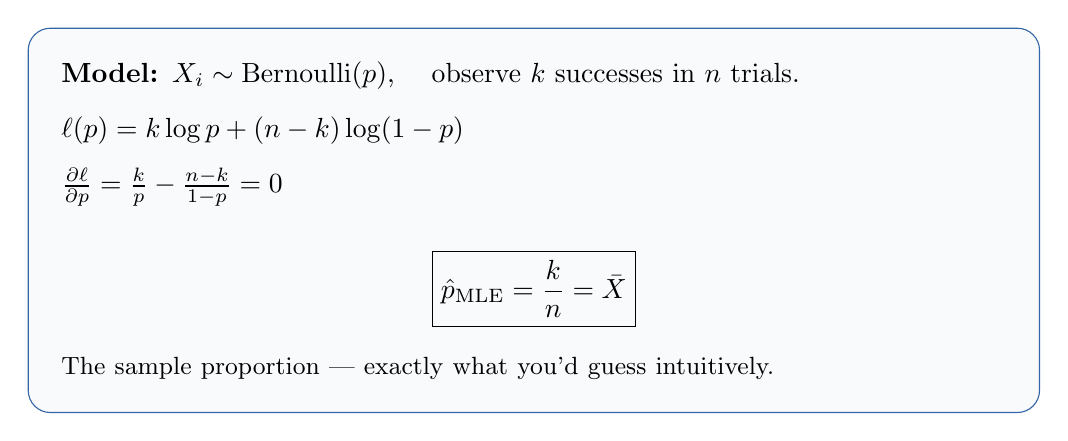
\begin{tikzpicture}
  \node[draw=popblue, fill=popblue!3, rounded corners=8pt, text width=12cm, align=left, inner sep=12pt] {
    \textbf{Model:} $X_i \sim \text{Bernoulli}(p)$, \quad observe $k$ successes in $n$ trials.\\[8pt]
    $\ell(p) = k\log p + (n-k)\log(1-p)$\\[8pt]
    $\frac{\partial\ell}{\partial p} = \frac{k}{p} - \frac{n-k}{1-p} = 0$\\[8pt]\pause
    $$\boxed{\hat{p}_{\text{MLE}} = \frac{k}{n} = \bar{X}}$$\\[4pt]
    \small The sample proportion --- exactly what you'd guess intuitively.
  };
\end{tikzpicture}
\end{center}
\end{frame}

\begin{frame}
\frametitle{MLE for Normal: Full Derivation}

\small
\textbf{Model:} $X_1, \ldots, X_n \overset{\text{iid}}{\sim} \mathcal{N}(\mu, \sigma^2)$, \;both $\mu$ and $\sigma^2$ unknown.

\vspace{0.1cm}
\textbf{Step 1.}\; Write the likelihood (product of $n$ Gaussian densities):
\vspace{-0.1cm}
$$L(\mu, \sigma^2) = \prod_{i=1}^n \frac{1}{\sqrt{2\pi\sigma^2}}\,\exp\!\!\left(-\frac{(X_i - \mu)^2}{2\sigma^2}\right)$$

\vspace{-0.3cm}\pause
\textbf{Step 2.}\; Take the log (product $\to$ sum):
\vspace{-0.15cm}
$$\ell(\mu, \sigma^2) = -\tfrac{n}{2}\log(2\pi) - \tfrac{n}{2}\log\sigma^2 - \frac{1}{2\sigma^2}\sum_{i=1}^n(X_i - \mu)^2$$

\vspace{-0.3cm}\pause
\textbf{Step 3.}\; Set $\dfrac{\partial\ell}{\partial\mu} = 0$: \quad $\dfrac{1}{\sigma^2}\displaystyle\sum_{i=1}^n(X_i - \mu) = 0 \quad\Longrightarrow\quad \boxed{\hat\mu_{\text{MLE}} = \bar{X}}$

\vspace{0.1cm}\pause
\textbf{Step 4.}\; Set $\dfrac{\partial\ell}{\partial(\sigma^2)} = 0$: \quad $-\dfrac{n}{2\sigma^2} + \dfrac{\sum(X_i - \bar{X})^2}{2\sigma^4} = 0$

\hfill$\Longrightarrow\quad \boxed{\hat\sigma^2_{\text{MLE}} = \frac{1}{n}\sum_{i=1}^n(X_i - \bar{X})^2}$\hspace{1.5cm}\null
\end{frame}

\begin{frame}
\frametitle{How Good Is the Normal MLE?}

\small
\begin{columns}[T]
\begin{column}{0.44\textwidth}
\textbf{For $\hat\mu = \bar{X}$:}
\begin{itemize}\setlength{\itemsep}{1pt}
  \item Bias $= 0$ \quad (unbiased)
  \item Var $= \sigma^2/n$
  \item MSE $= \sigma^2/n$
  \item[\textcolor{paramgreen}{\checkmark}] \textcolor{paramgreen}{$=$ CR bound --- \textbf{efficient!}}
\end{itemize}
\end{column}
\begin{column}{0.52\textwidth}
\textbf{For $\hat\sigma^2 = \frac{1}{n}\sum(X_i - \bar{X})^2$:}
\begin{itemize}\setlength{\itemsep}{1pt}
  \item Bias $= -\sigma^2/n$ \quad \textcolor{warnred}{(biased!)}
  \item Var $= 2(n{-}1)\sigma^4/n^2$
  \item MSE $= (2n{-}1)\sigma^4/n^2$
\end{itemize}
\end{column}
\end{columns}

\pause
\vspace{0.25cm}
\textbf{Compare with Bessel's $S^2 = \frac{1}{n-1}\sum(X_i - \bar{X})^2$} (unbiased):

\vspace{0.1cm}
\begin{center}\small
\renewcommand{\arraystretch}{1.3}
\begin{tabular}{@{}lcc@{}}
  & $\hat\sigma^2_{\text{MLE}}$ \;(divide by $n$) & $S^2$ \;(divide by $n{-}1$) \\
  \hline
  Bias & $-\sigma^2/n$ & $0$ \\
  MSE & $(2n{-}1)\sigma^4/n^2$ & $2\sigma^4/(n{-}1)$ \\
  \hline
\end{tabular}
\end{center}

\vspace{0.1cm}
\centering MSE$(\hat\sigma^2_{\text{MLE}}) <$ MSE$(S^2)$ \textbf{always!} \;The biased MLE wins on MSE (Lecture~3 tradeoff).
\end{frame}

\begin{frame}
\frametitle{From MLE to Machine Learning}

\small
In ML, we model: \;$y_i = f(\mathbf{x}_i;\, \mathbf{w}) + \varepsilon_i$, \quad $\varepsilon_i \overset{\text{iid}}{\sim} \mathcal{N}(0, \sigma^2)$

\vspace{0.15cm}
So $y_i \mid \mathbf{x}_i \sim \mathcal{N}\!\bigl(f(\mathbf{x}_i;\mathbf{w}),\; \sigma^2\bigr)$. \;The log-likelihood of $\mathbf{w}$:
\vspace{-0.15cm}
$$\ell(\mathbf{w}) = \underbrace{-\tfrac{n}{2}\log(2\pi\sigma^2)}_{\text{const w.r.t.\ }\mathbf{w}} - \frac{1}{2\sigma^2}\sum_{i=1}^n\bigl(y_i - f(\mathbf{x}_i;\mathbf{w})\bigr)^2$$

\vspace{-0.2cm}\pause
\begin{center}
$\max_{\mathbf{w}} \;\ell(\mathbf{w}) \quad\Longleftrightarrow\quad \min_{\mathbf{w}} \;\displaystyle\sum_{i=1}^n\bigl(y_i - f(\mathbf{x}_i;\mathbf{w})\bigr)^2 \quad=\quad$ \textbf{MSE loss!}
\end{center}

\vspace{0.15cm}
\begin{center}
\fcolorbox{violet1}{violet1!5}{\parbox{12cm}{\centering
  \textbf{Gaussian noise + MLE = Least Squares}\\[4pt]
  \small The MSE loss in machine learning is not arbitrary ---\\
  it is exactly \textbf{maximum likelihood under Gaussian noise}.\\[4pt]
  Linear regression, neural nets with MSE loss, OLS --- all are doing MLE.
}}
\end{center}

\vspace{0.1cm}
\centering\small Not just Gaussian --- every noise model gives a different loss function\ldots
\end{frame}

\begin{frame}
\frametitle{MLE and Cross-Entropy}

\small
Now: $y_i \in \{0,1\}$ \;\;(spam/not spam, click/no click, disease/healthy).

\vspace{0.15cm}
\textbf{Model:} \;$P(y_i = 1 \mid \mathbf{x}_i) = \sigma(\mathbf{w}^\top\!\mathbf{x}_i)$
\;\;where \;$\sigma(z) = \frac{1}{1 + e^{-z}}$ \;\;(logistic function)

\vspace{0.15cm}\pause
The log-likelihood:
\vspace{-0.15cm}
$$\ell(\mathbf{w}) = \sum_{i=1}^n \bigl[\, y_i \log \hat{p}_i + (1{-}y_i)\log(1{-}\hat{p}_i)\,\bigr] \qquad \hat{p}_i = \sigma(\mathbf{w}^\top\!\mathbf{x}_i)$$

\vspace{-0.25cm}\pause
\begin{center}
$\max_{\mathbf{w}}\;\ell(\mathbf{w}) \quad\Longleftrightarrow\quad \min_{\mathbf{w}} \;\underbrace{-\sum \bigl[\, y_i \log \hat{p}_i + (1{-}y_i)\log(1{-}\hat{p}_i)\,\bigr]}_{\text{\textbf{binary cross-entropy loss}}}$
\end{center}

\vspace{0.1cm}
\begin{center}
\fcolorbox{orange1}{orange1!5}{\parbox{12cm}{\centering\small
  \textbf{Bernoulli outcome + MLE = Cross-Entropy Loss}\\[3pt]
  Logistic regression, neural nets with sigmoid output --- all doing MLE.\\[3pt]
  \textbf{Gaussian} $\to$ MSE \quad|\quad \textbf{Bernoulli} $\to$ Cross-Entropy \quad|\quad \textbf{Laplace} $\to$ MAE
}}
\end{center}
\end{frame}

\begin{frame}
\frametitle{MLE: Poisson (Rare Events)}

\vspace{-0.1cm}
\begin{columns}[T]
\begin{column}{0.54\textwidth}
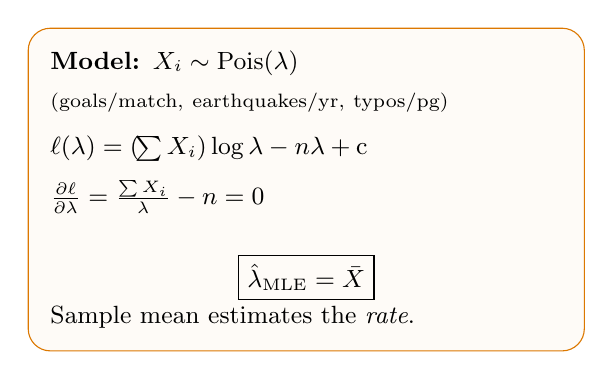
\begin{tikzpicture}
  \node[draw=orange1, fill=orange1!3, rounded corners=8pt, text width=6.5cm, align=left, inner sep=8pt, font=\small] {
    \textbf{Model:} $X_i \sim \text{Pois}(\lambda)$\\[3pt]
    {\scriptsize (goals/match, earthquakes/yr, typos/pg)}\\[6pt]
    $\ell(\lambda) = (\!\sum X_i)\log\lambda - n\lambda + \text{c}$\\[6pt]
    $\frac{\partial\ell}{\partial\lambda} = \frac{\sum X_i}{\lambda} - n = 0$\\[6pt]\pause
    $$\boxed{\hat{\lambda}_{\text{MLE}} = \bar{X}}$$\\[-2pt]
    \small Sample mean estimates the \textit{rate}.
  };
\end{tikzpicture}
\end{column}
\begin{column}{0.44\textwidth}
\vspace{0.1cm}
\begin{center}
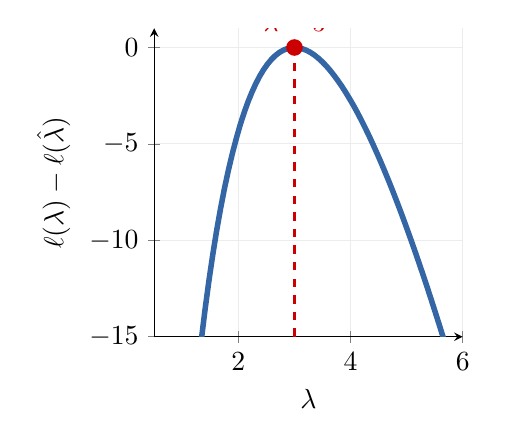
\begin{tikzpicture}
  \begin{axis}[
    width=5.5cm, height=5.5cm,
    xlabel={$\lambda$},
    ylabel={$\ell(\lambda) - \ell(\hat\lambda)$},
    xmin=0.5, xmax=6,
    ymin=-15, ymax=1,
    axis lines=left,
    grid=major, grid style={gray!15},
    every axis plot/.append style={line width=2pt, samples=80},
  ]
    % l(lambda) - l(3) = 60(ln(lambda)-ln(3)) - 20(lambda-3), n=20, sum=60
    \addplot[popblue, domain=0.5:6] {60*(ln(x)-ln(3)) - 20*(x-3)};

    % MLE marker
    \draw[very thick, sampred, dashed] (axis cs:3, -15) -- (axis cs:3, 0);
    \fill[sampred] (axis cs:3, 0) circle (3pt);
    \node[font=\small\bfseries, sampred, above] at (axis cs:3, 0.3) {$\hat\lambda = 3$};
  \end{axis}
\end{tikzpicture}
\end{center}
\footnotesize\centering Example: $n=20$, $\sum X_i = 60$
\end{column}
\end{columns}
\end{frame}

\begin{frame}
\frametitle{MLE: Exponential (Waiting Times)}
\begin{center}
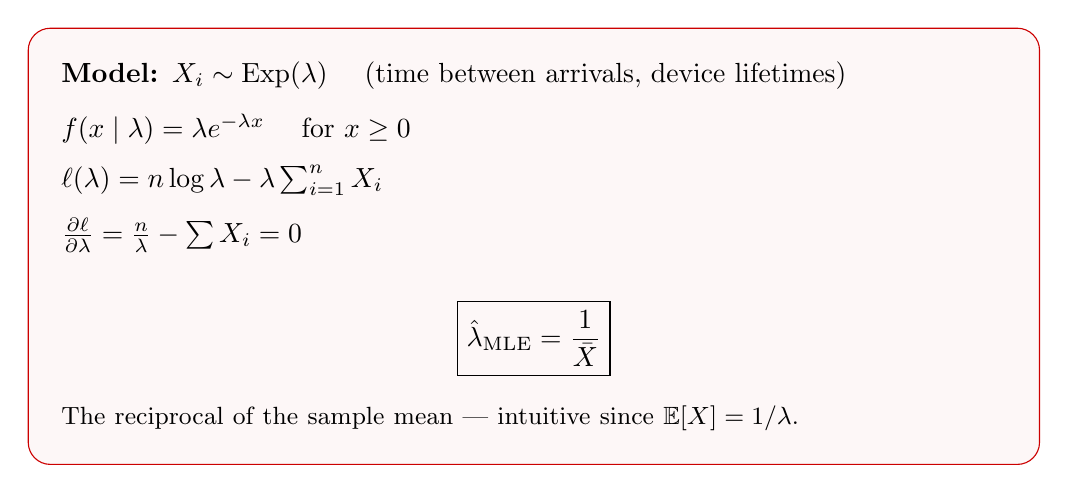
\begin{tikzpicture}
  \node[draw=sampred, fill=sampred!3, rounded corners=8pt, text width=12cm, align=left, inner sep=12pt] {
    \textbf{Model:} $X_i \sim \text{Exp}(\lambda)$ \quad (time between arrivals, device lifetimes)\\[8pt]
    $f(x \mid \lambda) = \lambda e^{-\lambda x}$ \quad for $x \ge 0$\\[6pt]
    $\ell(\lambda) = n\log\lambda - \lambda\sum_{i=1}^n X_i$\\[8pt]
    $\frac{\partial\ell}{\partial\lambda} = \frac{n}{\lambda} - \sum X_i = 0$\\[8pt]\pause
    $$\boxed{\hat{\lambda}_{\text{MLE}} = \frac{1}{\bar{X}}}$$\\[4pt]
    \small The reciprocal of the sample mean --- intuitive since $\mathbb{E}[X] = 1/\lambda$.
  };
\end{tikzpicture}
\end{center}
\end{frame}

\begin{frame}
\frametitle{MLE: Summary of Examples}
\begin{center}
\renewcommand{\arraystretch}{1.8}
\begin{tabular}{lccc}
  \textbf{Distribution} & \textbf{Parameter} & \textbf{MLE} & \textbf{Real-world use} \\
  \hline
  Bernoulli$(p)$ & $p$ & $\bar{X}$ & Coin fairness, conversion rates \\
  Normal$(\mu, \sigma^2)$ & $\mu, \sigma^2$ & $\bar{X}, \;\frac{1}{n}\sum(X_i-\bar{X})^2$ & Measurement error \\
  Poisson$(\lambda)$ & $\lambda$ & $\bar{X}$ & Count data, rare events \\
  Exponential$(\lambda)$ & $\lambda$ & $1/\bar{X}$ & Waiting times, lifetimes \\
  \hline
\end{tabular}
\end{center}

\vspace{0.3cm}
\small Notice: for exponential families, MLE often equals MoM! We'll see why shortly.
\end{frame}

\begin{frame}
\frametitle{MoM vs MLE: When to Use Which?}
\begin{center}
\small
\renewcommand{\arraystretch}{1.6}
\begin{tabular}{lcc}
  & \textbf{Method of Moments} & \textbf{Maximum Likelihood} \\
  \hline
  \textbf{Idea} & Match sample moments & Maximize data probability \\
  \textbf{Computation} & Usually algebraic & May need optimization \\
  \textbf{Efficiency} & Generally \textcolor{warnred}{less efficient} & \textcolor{paramgreen}{Asymptotically optimal} \\
  \textbf{Impossible values?} & \textcolor{warnred}{Can happen} ($\hat\sigma^2 < 0$) & \textcolor{paramgreen}{Respects constraints} \\
  \textbf{Invariance} & \textcolor{warnred}{No} & \textcolor{paramgreen}{Yes} ($g(\hat\theta)$ is MLE of $g(\theta)$) \\
  \textbf{Exp.\ family} & Often \textcolor{paramgreen}{same as MLE} & Always uses suff.\ stat \\
  \hline
\end{tabular}
\end{center}

\vspace{0.3cm}
\begin{center}
\fcolorbox{popblue}{popblue!5}{\parbox{11cm}{\centering\small
  \textbf{Rule of thumb:} Use MLE when you can (it's optimal).\\
  Use MoM as a quick starting point, or when MLE has no closed form.
}}
\end{center}
\end{frame}

% ============================================================
\section{MLE Properties}

\begin{frame}
\frametitle{Invariance Property}
\begin{center}
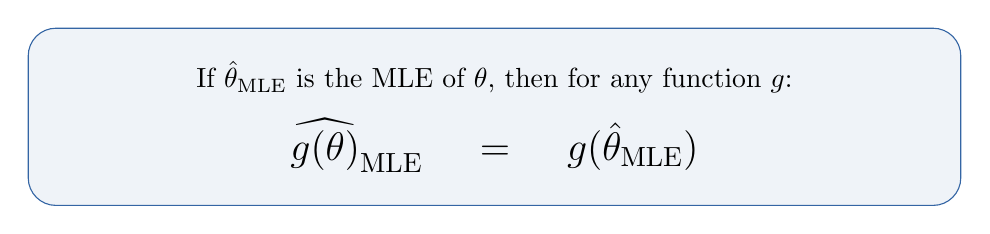
\begin{tikzpicture}
  \node[draw=popblue, fill=popblue!8, rounded corners=10pt, text width=11cm, align=center, inner sep=12pt] {
    If $\hat{\theta}_{\text{MLE}}$ is the MLE of $\theta$, then for any function $g$:\\[8pt]
    {\Large $\widehat{g(\theta)}_{\text{MLE}} = g(\hat{\theta}_{\text{MLE}})$}
  };
\end{tikzpicture}
\end{center}

\vspace{0.2cm}
\pause
\begin{columns}[T]
\begin{column}{0.50\textwidth}
\textbf{Example:}
\begin{itemize}\setlength{\itemsep}{2pt}
  \item MLE of $\lambda$ for Exp is $\hat{\lambda} = 1/\bar{X}$
  \item Want MLE of mean $\mu = 1/\lambda$?
  \item Apply $g(\lambda) = 1/\lambda$:\;\;$\hat{\mu} = \bar{X}$ \;\textcolor{paramgreen}{$\checkmark$}
\end{itemize}

\vspace{0.15cm}
\small This doesn't hold for MoM or other estimators in general.
\end{column}
\begin{column}{0.48\textwidth}
\begin{center}
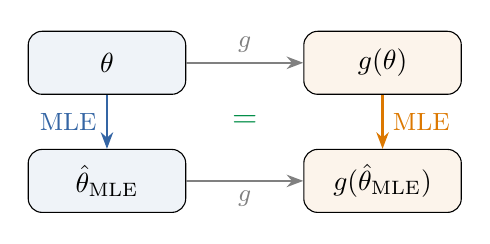
\begin{tikzpicture}[
  box/.style={draw, rounded corners=5pt, minimum width=2cm, minimum height=0.8cm, align=center, inner sep=4pt, font=\normalsize},
  arr/.style={-{Stealth[length=6pt]}, thick}
]
  \node[box, fill=popblue!8] (theta) at (0, 1.5) {$\theta$};
  \node[box, fill=orange1!8] (gtheta) at (3.5, 1.5) {$g(\theta)$};
  \node[box, fill=popblue!8] (thetahat) at (0, 0) {$\hat\theta_{\text{MLE}}$};
  \node[box, fill=orange1!8] (gthetahat) at (3.5, 0) {$g(\hat\theta_{\text{MLE}})$};

  \draw[arr, gray] (theta) -- (gtheta) node[midway, above, font=\small] {$g$};
  \draw[arr, popblue] (theta) -- (thetahat) node[midway, left, font=\small] {MLE};
  \draw[arr, orange1] (gtheta) -- (gthetahat) node[midway, right, font=\small] {MLE};
  \draw[arr, gray] (thetahat) -- (gthetahat) node[midway, below, font=\small] {$g$};

  \node[font=\large\bfseries, paramgreen] at (1.75, 0.75) {$=$};
\end{tikzpicture}
\end{center}
\end{column}
\end{columns}
\end{frame}

\begin{frame}
\frametitle{Identifiability}
\begin{center}
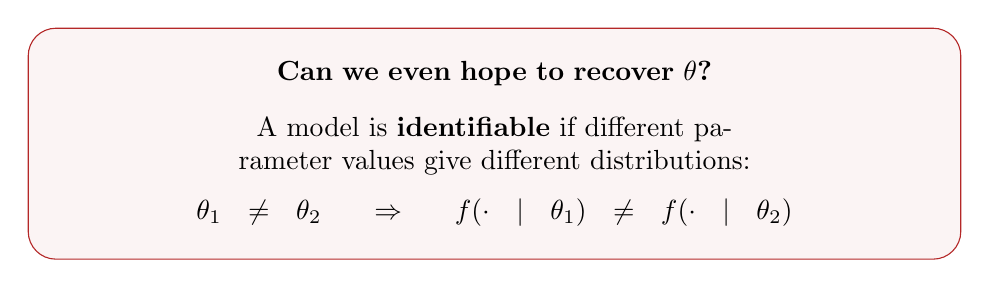
\begin{tikzpicture}
  \node[draw=warnred, fill=warnred!5, rounded corners=10pt, text width=11cm, align=center, inner sep=12pt] {
    \textbf{Can we even hope to recover $\theta$?}\\[8pt]
    A model is \textbf{identifiable} if different parameter values give different distributions:\\[6pt]
    $\theta_1 \ne \theta_2 \;\Rightarrow\; f(\cdot \mid \theta_1) \ne f(\cdot \mid \theta_2)$
  };
\end{tikzpicture}
\end{center}

\vspace{0.4cm}
\textbf{When it fails:}
\begin{itemize}
  \item \textbf{Mixture models:} swapping component labels gives the same distribution
  \item \textbf{Overparameterized models:} more parameters than the data can distinguish
  \item \textbf{Symmetric likelihoods:} multiple maxima, MLE is not unique
\end{itemize}

\vspace{0.3cm}
\small If the model isn't identifiable, no amount of data will help.
\end{frame}

\begin{frame}
\frametitle{Visualizing Non-Identifiability}
\begin{center}
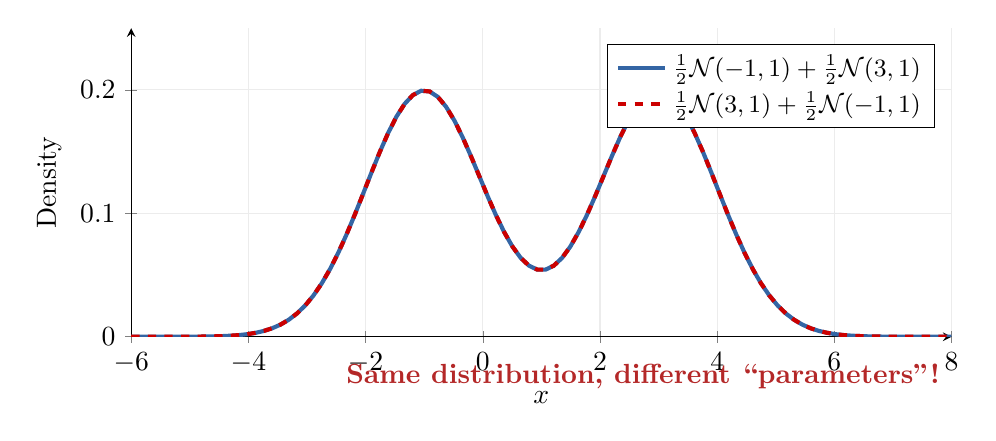
\begin{tikzpicture}
  \begin{axis}[
    width=12cm, height=5.5cm,
    xlabel={$x$},
    ylabel={Density},
    xmin=-6, xmax=8,
    ymin=0, ymax=0.25,
    axis lines=left,
    grid=major, grid style={gray!15},
    every axis plot/.append style={line width=1.5pt, samples=100},
    legend style={at={(0.98,0.95)}, anchor=north east, font=\small}
  ]
    % Same mixture, two parameterizations
    \addplot[popblue, domain=-6:8] {0.5 * exp(-(x+1)^2/2)/sqrt(2*pi) + 0.5 * exp(-(x-3)^2/2)/sqrt(2*pi)};
    \addlegendentry{$\frac{1}{2}\mathcal{N}(-1,1) + \frac{1}{2}\mathcal{N}(3,1)$}

    \addplot[sampred, dashed, domain=-6:8] {0.5 * exp(-(x-3)^2/2)/sqrt(2*pi) + 0.5 * exp(-(x+1)^2/2)/sqrt(2*pi)};
    \addlegendentry{$\frac{1}{2}\mathcal{N}(3,1) + \frac{1}{2}\mathcal{N}(-1,1)$}
  \end{axis}

  \node[font=\normalsize\bfseries, text=warnred] at (6.5, -0.5) {Same distribution, different ``parameters''!};
\end{tikzpicture}
\end{center}
\end{frame}

% ============================================================
\section{MLE Meets Lecture 3}

\begin{frame}
\frametitle{MLE and Sufficient Statistics}

\small
In Lecture~3 we learned: a \textbf{sufficient statistic} $T(\mathbf{X})$ captures everything about $\theta$.

\vspace{0.15cm}
\begin{center}
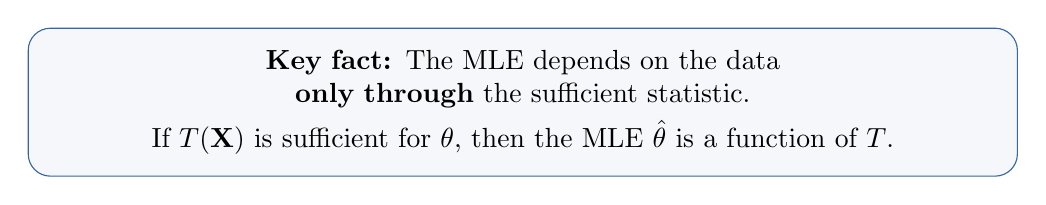
\begin{tikzpicture}
  \node[draw=popblue, fill=popblue!5, rounded corners=8pt, text width=12cm, align=center, inner sep=8pt] {
    \textbf{Key fact:} The MLE depends on the data \textbf{only through} the sufficient statistic.\\[4pt]
    If $T(\mathbf{X})$ is sufficient for $\theta$, then the MLE $\hat\theta$ is a function of $T$.
  };
\end{tikzpicture}
\end{center}

\vspace{0.1cm}
\textbf{Check our examples:}
\vspace{0.05cm}

\renewcommand{\arraystretch}{1.4}
\begin{center}
\begin{tabular}{lccc}
  \textbf{Model} & \textbf{Suff.\ stat} $T$ & \textbf{MLE} & \textbf{Function of $T$?} \\
  \hline
  $\text{Bern}(p)$ & $\sum X_i$ & $\bar{X} = T/n$ & \textcolor{paramgreen}{\checkmark} \\
  $N(\mu, \sigma_0^2)$ & $\sum X_i$ & $\bar{X} = T/n$ & \textcolor{paramgreen}{\checkmark} \\
  $\text{Pois}(\lambda)$ & $\sum X_i$ & $\bar{X} = T/n$ & \textcolor{paramgreen}{\checkmark} \\
  $\text{Exp}(\lambda)$ & $\sum X_i$ & $1/\bar{X} = n/T$ & \textcolor{paramgreen}{\checkmark} \\
  \hline
\end{tabular}
\end{center}

\vspace{0.1cm}
\begin{center}
\small No coincidence --- MLE \textbf{always} uses sufficient statistics. No information is wasted.
\end{center}
\end{frame}

\begin{frame}
\frametitle{MLE in Exponential Families}

\small
Recall the \textbf{exponential family} form from Lecture~3:
$\;f(x \mid \theta) = h(x)\exp\!\big(\eta(\theta)\,T(x) - A(\theta)\big)$

\vspace{0.2cm}
For $n$ i.i.d.\ observations, the log-likelihood is:
$$\ell(\theta) = \eta(\theta)\sum_{i=1}^n T(X_i) - nA(\theta) + \text{const}$$

Setting the derivative to zero:
$$\eta'(\theta)\sum_{i=1}^n T(X_i) = n A'(\theta)$$

\vspace{0.1cm}
\begin{center}
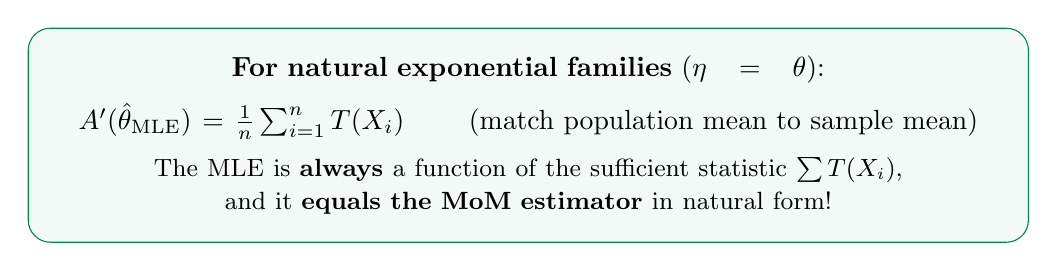
\begin{tikzpicture}
  \node[draw=paramgreen, fill=paramgreen!5, rounded corners=8pt, text width=12cm, align=center, inner sep=10pt] {
    \textbf{For natural exponential families} ($\eta = \theta$):\\[6pt]
    $A'(\hat\theta_{\text{MLE}}) = \frac{1}{n}\sum_{i=1}^n T(X_i)$ \qquad (match population mean to sample mean)\\[6pt]
    \small The MLE is \textbf{always} a function of the sufficient statistic $\sum T(X_i)$,\\
    and it \textbf{equals the MoM estimator} in natural form!
  };
\end{tikzpicture}
\end{center}
\end{frame}

\begin{frame}
\frametitle{Why MLE Works: The Big Theoretical Guarantees}

\small
Under regularity conditions (Lecture~4), MLE has remarkable properties:

\vspace{0.15cm}
\begin{center}
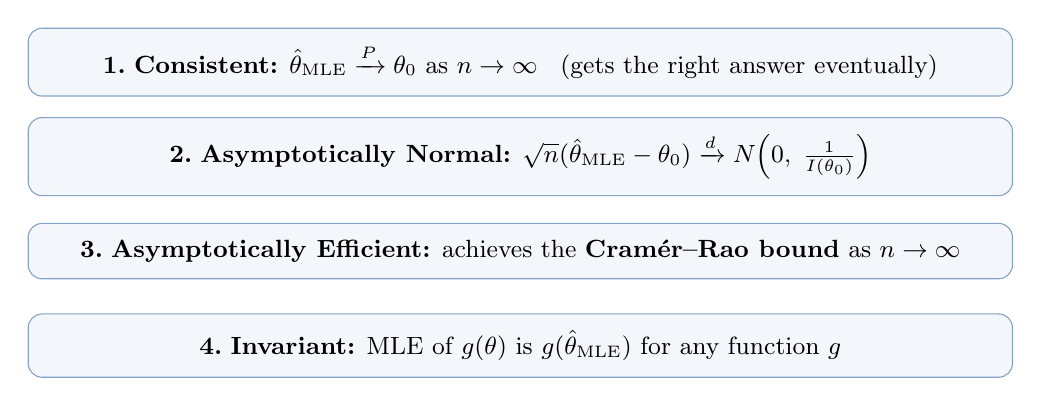
\begin{tikzpicture}[
  gbox/.style={draw=popblue!60, fill=popblue!6, rounded corners=5pt, minimum width=12.5cm, align=left, inner sep=6pt, font=\small}
]
  \node[gbox] at (0, 2.4) {\textbf{1.\;Consistent:} $\hat\theta_{\text{MLE}} \xrightarrow{P} \theta_0$ as $n \to \infty$ \;\;(gets the right answer eventually)};
  \node[gbox] at (0, 1.2) {\textbf{2.\;Asymptotically Normal:} $\sqrt{n}(\hat\theta_{\text{MLE}} - \theta_0) \xrightarrow{d} N\!\left(0,\; \frac{1}{I(\theta_0)}\right)$};
  \node[gbox] at (0, 0) {\textbf{3.\;Asymptotically Efficient:} achieves the \textbf{Cram\'er--Rao bound} as $n \to \infty$};
  \node[gbox] at (0, -1.2) {\textbf{4.\;Invariant:} MLE of $g(\theta)$ is $g(\hat\theta_{\text{MLE}})$ for any function $g$};
\end{tikzpicture}
\end{center}

\pause
\vspace{0.15cm}
\begin{center}
\fcolorbox{violet1}{violet1!5}{\parbox{11cm}{\centering\small
  \textbf{Translation:} With enough data, MLE is approximately unbiased,\\
  approximately normal, and \textbf{no other estimator can do better}.\\[3pt]
  This is why MLE is the default method in statistics and machine learning.
}}
\end{center}
\end{frame}

\begin{frame}
\frametitle{Asymptotic Normality: Seeing It}

\small
As $n$ grows, the sampling distribution of the MLE converges to a Normal centered at the truth:

\vspace{0.1cm}
\begin{center}
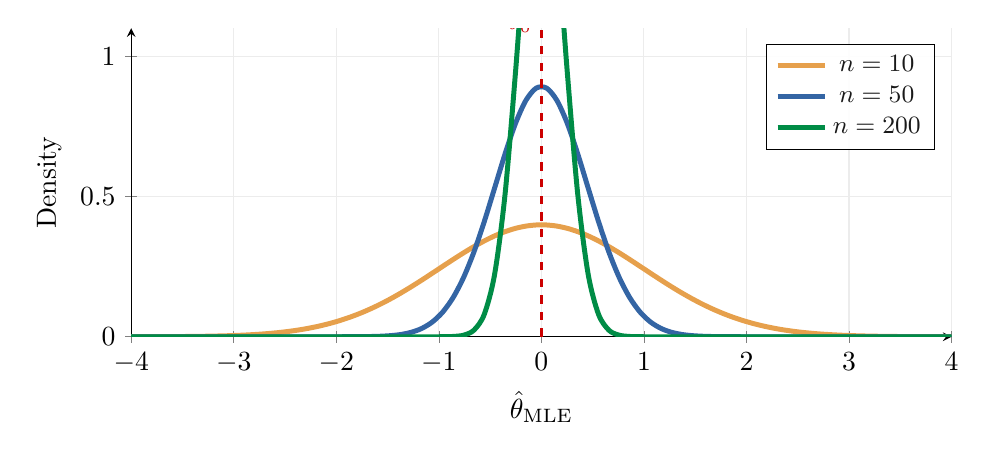
\begin{tikzpicture}
  \begin{axis}[
    width=12cm, height=5.5cm,
    xlabel={$\hat\theta_{\text{MLE}}$},
    ylabel={Density},
    xmin=-4, xmax=4,
    ymin=0, ymax=1.1,
    axis lines=left,
    grid=major, grid style={gray!15},
    every axis plot/.append style={line width=1.8pt, smooth, samples=80},
    legend style={at={(0.98,0.95)}, anchor=north east, font=\small, fill=white, fill opacity=0.9},
  ]
    % n=10: wide
    \addplot[orange1!70, domain=-4:4] {1/sqrt(2*pi*1)*exp(-x^2/(2*1))};
    \addlegendentry{$n = 10$}

    % n=50: medium
    \addplot[popblue, domain=-4:4] {1/sqrt(2*pi*0.2)*exp(-x^2/(2*0.2))};
    \addlegendentry{$n = 50$}

    % n=200: tight
    \addplot[paramgreen, domain=-4:4] {1/sqrt(2*pi*0.05)*exp(-x^2/(2*0.05))};
    \addlegendentry{$n = 200$}

    % True value
    \draw[dashed, thick, sampred] (axis cs:0, 0) -- (axis cs:0, 1.1);
    \node[font=\small\bfseries, sampred, above left] at (axis cs:0, 1.05) {$\theta_0$};
  \end{axis}
\end{tikzpicture}
\end{center}

\vspace{-0.1cm}
\begin{center}
\small Variance shrinks as $\frac{1}{n\,I(\theta_0)}$\,: more data $\Rightarrow$ tighter bell $\Rightarrow$ more precise estimate.\\
With $n = 200$ observations, MLE is practically pinpointed at the truth.
\end{center}
\end{frame}

\begin{frame}
\frametitle{MLE Achieves the Cram\'er--Rao Bound}

\small
From Lecture~4, the \textbf{CR bound}: $\text{Var}(\hat\theta) \geq \frac{1}{n\,I(\theta)}$ for unbiased estimators.

\vspace{0.2cm}
\textbf{Does MLE hit this bound?}

\vspace{0.2cm}
\begin{center}
\renewcommand{\arraystretch}{1.6}
\begin{tabular}{lcccc}
  \textbf{Model} & \textbf{MLE} & $\text{Var}(\hat\theta_{\text{MLE}})$ & \textbf{CR bound} & \textbf{Efficient?} \\
  \hline
  $\text{Bern}(p)$ & $\bar{X}$ & $\frac{p(1-p)}{n}$ & $\frac{p(1-p)}{n}$ & \textcolor{paramgreen}{\textbf{Yes}} \\[3pt]
  $N(\mu, \sigma_0^2)$ & $\bar{X}$ & $\frac{\sigma_0^2}{n}$ & $\frac{\sigma_0^2}{n}$ & \textcolor{paramgreen}{\textbf{Yes}} \\[3pt]
  $\text{Pois}(\lambda)$ & $\bar{X}$ & $\frac{\lambda}{n}$ & $\frac{\lambda}{n}$ & \textcolor{paramgreen}{\textbf{Yes}} \\
  \hline
\end{tabular}
\end{center}

\vspace{0.2cm}
\begin{center}
\fcolorbox{paramgreen}{paramgreen!5}{\parbox{11cm}{\centering\small
  For \textbf{exponential families}, the MLE of the natural parameter is efficient (hits the CR bound exactly). For other models, MLE is \textbf{asymptotically} efficient --- it approaches the bound as $n \to \infty$.
}}
\end{center}
\end{frame}

\begin{frame}
\frametitle{When MLE Goes Wrong}

\small
MLE has great asymptotic theory, but several things can go wrong:

\vspace{0.15cm}
\begin{itemize}\setlength{\itemsep}{4pt}
  \item \textbf{Small samples:} MLE is asymptotic --- can be poor for small $n$.\\
    {\footnotesize Example: 0 heads in 3 flips $\Rightarrow$ $\hat{p}_{\text{MLE}} = 0$. Surely too extreme!}

  \pause
  \item \textbf{Boundary of parameter space:} $\text{Uniform}(0, \theta)$ $\Rightarrow$ $\hat\theta = X_{(n)}$.\\
    {\footnotesize Always underestimates: bias $= -\theta/(n{+}1)$, not the usual $O(1/n)$.}

  \pause
  \item \textbf{Neyman--Scott problem:} Too many nuisance parameters $\Rightarrow$ \textbf{inconsistent} MLE.\\
    {\footnotesize $n$ groups with 2 obs each, own mean $\mu_i$: MLE of $\sigma^2$ converges to $\sigma^2/2$!}

  \pause
  \item \textbf{Overfitting:} Flexible models memorize noise.\\
    {\footnotesize Degree-20 polynomial through 25 points $\Rightarrow$ wild oscillations.}
\end{itemize}

\vspace{0.15cm}
\begin{center}
\fcolorbox{violet1}{violet1!5}{\parbox{11cm}{\centering\small
  \textbf{Common cure:} Add a prior $\to$ MAP estimation (Lecture~6).\\
  Prior = regularization = controlled bias toward simpler models.
}}
\end{center}
\end{frame}

\begin{frame}
\frametitle{When There's No Closed Form}

\small
Many models (logistic regression, mixtures, neural nets) require \textbf{numerical} optimization.

\vspace{0.1cm}
\begin{columns}[T]
\begin{column}{0.42\textwidth}
\begin{center}
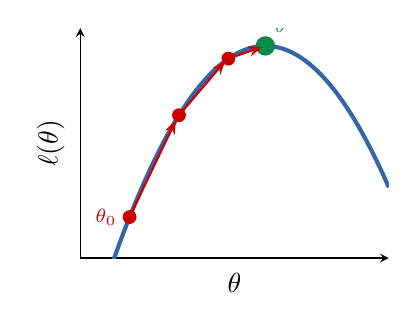
\begin{tikzpicture}
  \begin{axis}[
    width=5.5cm, height=4.5cm,
    xlabel={$\theta$},
    ylabel={$\ell(\theta)$},
    xmin=0, xmax=5, ymin=-12, ymax=1,
    axis lines=left,
    grid=major, grid style={gray!15},
    xtick=\empty, ytick=\empty,
  ]
    \addplot[popblue, line width=1.5pt, domain=0.3:5, samples=80] {-2*(x-3)^2};

    \fill[sampred] (axis cs:0.8, -9.68) circle (2.5pt);
    \fill[sampred] (axis cs:1.6, -3.92) circle (2.5pt);
    \fill[sampred] (axis cs:2.4, -0.72) circle (2.5pt);
    \fill[paramgreen] (axis cs:3.0, 0) circle (3.5pt);

    \draw[thick, sampred, -{Stealth[length=5pt]}] (axis cs:0.8, -9.68) -- (axis cs:1.55, -4.2);
    \draw[thick, sampred, -{Stealth[length=5pt]}] (axis cs:1.6, -3.92) -- (axis cs:2.35, -0.85);
    \draw[thick, sampred, -{Stealth[length=5pt]}] (axis cs:2.4, -0.72) -- (axis cs:2.95, -0.05);

    \node[font=\scriptsize, sampred, left] at (axis cs:0.75, -9.68) {$\theta_0$};
    \node[font=\scriptsize\bfseries, paramgreen, above right] at (axis cs:3.0, 0.2) {$\hat\theta$};
  \end{axis}
\end{tikzpicture}
\end{center}
\end{column}
\begin{column}{0.55\textwidth}
\textbf{Gradient ascent:}
$$\theta_{t+1} = \theta_t + \alpha \cdot \ell'(\theta_t)$$

\small Follow the slope uphill. The default in deep learning.

\vspace{0.2cm}
\textbf{Newton--Raphson:}
$$\theta_{t+1} = \theta_t - \frac{\ell'(\theta_t)}{\ell''(\theta_t)}$$

\small Uses curvature ($\ell'' \leftrightarrow$ Fisher info) for smarter steps.

\vspace{0.15cm}
\footnotesize In Python: \texttt{scipy.optimize.minimize}
\end{column}
\end{columns}
\end{frame}

% ============================================================
\section{Practical}

\begin{frame}
\frametitle{Practical: Implement MLE}
\begin{center}
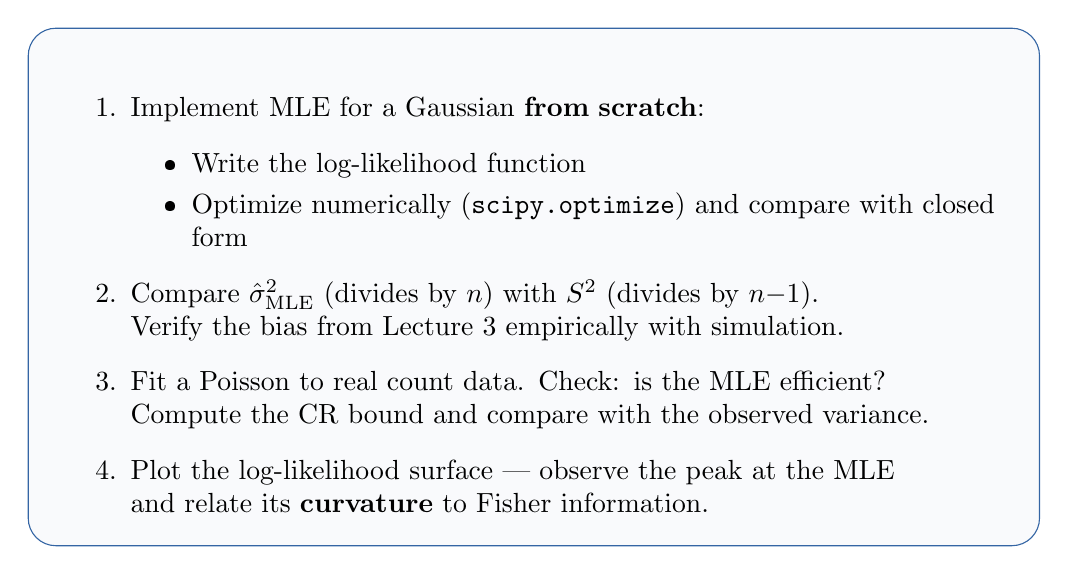
\begin{tikzpicture}
  \node[draw=popblue, fill=popblue!3, rounded corners=10pt, text width=12cm, align=left, inner sep=12pt] {
    \begin{enumerate}\setlength{\itemsep}{4pt}
      \item Implement MLE for a Gaussian \textbf{from scratch}:
        \begin{itemize}\setlength{\itemsep}{1pt}
          \item Write the log-likelihood function
          \item Optimize numerically (\texttt{scipy.optimize}) and compare with closed form
        \end{itemize}
      \item Compare $\hat\sigma^2_{\text{MLE}}$ (divides by $n$) with $S^2$ (divides by $n{-}1$).\\
        Verify the bias from Lecture~3 empirically with simulation.
      \item Fit a Poisson to real count data. Check: is the MLE efficient?\\
        Compute the CR bound and compare with the observed variance.
      \item Plot the log-likelihood surface --- observe the peak at the MLE\\
        and relate its \textbf{curvature} to Fisher information.
    \end{enumerate}
  };
\end{tikzpicture}
\end{center}
\end{frame}

\begin{frame}
\frametitle{Homework}
\begin{enumerate}
  \item Derive the MLE for $\text{Geometric}(p)$: $\;f(x \mid p) = (1-p)^{x-1}p$, $\;x = 1, 2, \ldots$\\
    Is this MLE unbiased? Is it efficient (check against the CR bound)?

  \vspace{0.15cm}
  \item For $X_1, \ldots, X_n \sim N(\mu, \sigma^2)$, show that $\hat\sigma^2_{\text{MLE}} = \frac{1}{n}\sum(X_i - \bar{X})^2$\\
    equals the MoM estimator. Why is this not a coincidence? (Hint: exponential family.)

  \vspace{0.15cm}
  \item Show that the MLE for $\text{Uniform}(0, \theta)$ is $\hat\theta = X_{(n)} = \max(X_1, \ldots, X_n)$.\\
    Is this unbiased? Is it consistent? (Note: this is \textbf{not} an exponential family!)

  \vspace{0.15cm}
  \item Simulate $n = 50$ samples from $\text{Poisson}(\lambda = 3)$ and compute the MLE.\\
    Repeat 10{,}000 times. Verify: (a) $\hat\lambda$ is approximately unbiased, (b)~$\text{Var}(\hat\lambda) \approx \lambda/n$.
\end{enumerate}
\end{frame}

\begin{frame}
\begin{center}
  {\Huge\bfseries\textcolor{popblue}{Questions?}}

  \vspace{1cm}

  {\large Next: MAP estimation, priors, and the Bayesian perspective}
\end{center}
\end{frame}

\end{document}
